\chapter{The Image Annotation Problem}%
\label{cha:the_image_annotation_problem}

\adjustmtc
\minitoc%

\newpage
In this chapter we will discuss the concept of image annotation,
and review the body of work that have been researched in this domain.
But first, what is image annotation?
Fundamentally, it is the process of augmenting an image with information.
This information can be of various nature,
typically provided by a human operator, also called annotator.
We review the different types of annotations in Section~\ref{sec:annotation-types}.

We could consider image captioning as the first historical example of image annotation,
simply consisting in adding a caption to an image.
We could also consider photogrammetry as a form of image annotation which,
long before digital images even existed,
is the process of measuring distances and lengths of the real world from 2D images.
It requires annotating these distances and lengths in the image space,
before inferring the values in the real world.
Early techniques in the old cinema also involved
manually editing the filmstrip to create special effects, which is a form of annotation.

Digital imaging has progressively brought new needs for image annotation.
The first digital image was scanned from a photograph in 1957 by Russell Kirsch,
and the first digital camera was built in 1975 by Kodak engineer Steve Sasson.
Commercial models of digital cameras became really available in the 1990s,
and from then the volume of digital images produced grew exponentially every year.
Meanwhile the field of computer vision, aiming at understanding those images,
also developed its own research community.
The highly influencial journal \textit{IEEE Transactions on Pattern Analysis
and Machine Intelligence} (TPAMI) was for example created in 1979.
Computer vision is also related to the field of machine learning,
which designates a class of algorithms in which a model learns from experience,
materialized by data samples.
One sub-domain of machine learning, called \textit{supervised} machine learning,
requires in particular annotated samples,
meaning that a label should be assigned to each piece of data before
an algorithm can be trained to predict these labels.
Supervised machine learning gained traction in the 1990s during which
some applications reached high enough maturity to be exploited commercially.
A famous example of this is the digit recognition algorithm from
Lecun et al.~\cite{lecun1998gradient} which was used by AT\&T
to automatically process cheques in ATM (see Figure~\ref{fig:lenet}).
A nowadays popular dataset,
called MNIST (Mixed National Institute of Standards and Technology)
was created for this work;
this dataset associates labels (digits, from 0 to 9)
to $28\times 28$ pixel images of handwritten figures.

\begin{figure}[ht]
\centering
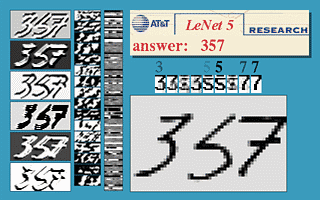
\includegraphics[width=0.5\columnwidth]{assets/img/lenet-results.png}
\caption{Illustration of the digit recognition algorithm from Lecun et al.\ \cite{lecun1998gradient}}%
\label{fig:lenet}
\end{figure}

This dataset illustrates how image annotation could be used
to produce desirable applications, and is only a small example of what
has now become a classic pipeline to solve problems in the computer vision community.
Since image annotation has become key in this community,
this chapter focuses on computer vision but
the machine learning pipeline we mention is also used in many other problems
such as audio or natural language processing.

Theoretical results in machine learning postulate that
problems of great complexity could be adressed with this technique,
provided that (i) there exists a model of sufficient capacity
to cope with the problem complexity,
and (ii) a sufficiently large sample of annotated data is available.
Some thresholds have been established by the community to estimate
what ``sufficiently large'' means~\cite{raudys1991small, jain198239},
but computer vision problems typically requires millions
of annotated images to be solved with an acceptable performance.
Models relying on deep neural networks are nowadays
the most popular techniques in machine learning,
but other models, such as deep random forests,
used in the human body pose estimation embedded in the Kinect~\cite{shotton2011real},
may still be considered depending on the application.
Note that while gathering more and more data is the current trend in computer vision,
an important field of research conversely focuses on learning on few samples;
this field regroups the notions of semi-supervised learning,
weakly-supervised learning, one-shot and few-shots learning, etc.

In what follows, we will review the computer vision problems for which large datasets,
often combined with (deep) machine learning techniques,
have recently significantly improved the state-of-the-art.
We will then discuss the process of gathering these annotations,
focusing on some key aspects such as expert vs.\ non-expert annotations, quality control, etc.
We will end with a presentation of possible interactions that can be used to annotate an image.

\section{Computer vision problems that require annotation}%
\label{sec:cv_annot}

\subsection{Image classification}

Image understanding forms a category of hard problems, but among them,
what could be considered the simplest one is \textit{image classification}.
Classifying an image consists in assigning it
labels describing either the type of scene it depicts
such as interior, exterior, beach, mountain, forest, city,
or the objects that are displayed, sorted by importance.
This task requires an advanced understanding of the images.

In fact, two of the most important challenges in computer vision
have highlighted this task as one of the main problem to be solved.
The first one, Pattern Analysis, Statistical Modelling and Computational
Learning Visual Objects Challenge, often called PASCAL VOC~\cite{Everingham10},
has run from 2005 to 2012 and figured at its peak 11,530 images depicting 20 classes.
It is interesting to note that this challenge coincides in time
with the rise of machine learning popularity in the computer vision community.
In a way, PASCAL VOC has been both a marker and a catalyzer of the importance
of machine learning in image processing problems.
PASCAL VOC stopped in 2012 sadly due to
the passing of one of its most invested organizers, Mark Everingham,
as well as due to the growing importance of a much larger challenge:
the ImageNet Large Scale Visual Recognition Challenge (ILSVRC).

ILSVRC~\cite{ILSVRC15} started in 2010,
motivated by the goal to solve larger scale problems.
ILSVRC relies on a gigantic dataset called ImageNet,
that originally intended to match a natural language
dataset called WordNet~\cite{miller1995wordnet}.
WordNet is a database of english words, grouped into sets of synonyms called synsets.
The goal of ImageNet is to provide a set of images to describe each of these synsets.
As of December 4th 2019, ImageNet displays 14,197,122 images that depict 21,841 different synsets.

We should also mention a parallel effort funded by
the Canadian Institute for Advanced Research,
which led to the creation of CIFAR-10 and CIFAR-100.
Those datasets contain images of size $32 \times 32$ collected
over various Web images searching tools,
and classified under 10 and 100 classes respectively.
ImageNet and CIFAR-100 are often both used to assess the performance of image classifiers.

While many subsequent work have further improved state-of-the-art classification results,
we could synthesize the progress in classification by citing two papers.
The first one from Krizhevsky et al.\ in 2012~\cite{krizhevsky2012imagenet},
nicknamed AlexNet, was probably key in the rise of deep learning that followed.
AlexNet won the ILSVRC 2012 challenge by a large margin,
starting the trend of using deep neural networks to solve computer vision problems.
The second paper from He et al.\ in 2016 and often called ResNet~\cite{he2016deep},
introduced residual blocks through skip connections
to ease the training of very deep neural networks, up to 1000 layers!
The 152 layers version of ResNet won the ILSVRC 2015 challenge
by reaching an error rate so low that
it could be considered below the average human performance.
The general trend in subsequent work has been to reach comparable
or higher performance than ResNet while
reducing the number of parameters and operations to a minimum.

\begin{table}
\centering
\caption{Datasets for image classification and their characteristics.}
\begin{tabular}{lllll}
	Dataset & Year & \# classes & \# images &  annotation process \\
	\midrule
	PASCAL VOC~\cite{Everingham10} & 2005 -- 2012 & 20 & 11.5k &  In-house \\
	ESP Game~\cite{von2005esp} & unreported & any & 100k &  ESP Game players \\
	CIFAR-10~\cite{krizhevsky2009learning} & 2009 & 10 & 60k  & Recruited students \\
	CIFAR-100~\cite{krizhevsky2009learning} & 2009 & 100 & 60k  & Recruited students \\
	SUN397~\cite{xiao2010sun} & 2010 & 397 & 130k &   \\
	ImageNet~\cite{ILSVRC15} & 2010 -- now & 21k & 14M &  Mechanical Turk \\
	Open Images~\cite{OpenImages, OpenImages2} & 2016 -- now & 8.5k & 9.2M & \makecell[l]{In-house and\\Crowdsource app} \\
\end{tabular}%
\label{tab:classification_ds}
\end{table}

\subsection{Image captioning}

Another important topic, that extends in a sense the image classification problem,
is the one of \textit{image captioning}.
It consists in describing an image with a set of sentences.
Image captioning is a much harder problem than classification,
because captions require a higher level of image understanding as well as
natural language capabilities to generate valid sentences.
In terms of annotations, it is also much longer to caption
an image than just assigning it a class.
Another difficulty for data gathering is the quality check of the annotations,
since two sentences from two different users may be
completely different but still convey the same semantic meaning.

\begin{table}
\centering
\caption{Datasets for image captioning and their characteristics.}
\begin{tabular}{lllll}
	Dataset & Year & \# captions & \# images & annotation process \\
	\midrule
	Flickr30k~\cite{flickr30k} & 2014 & 150k & 30k & Mechanical Turk \\
	MS COCO~\cite{chen2015microsoft} & 2015 & 1M & 164k & Mechanical Turk \\
	Conceptual Captions~\cite{sharma-etal-2018-conceptual} & 2018 & 3.3M & 3.3M & Web crawling \\
	\texttt{nocaps}~\cite{agrawal2019nocaps} & 2019 &  166k & 15k & Mechanical Turk \\
\end{tabular}%
\label{tab:caption_ds}
\end{table}

The datasets introduced in Table~\ref{tab:caption_ds} have brought
large enough sets of examples to efficiently train deep neural networks.
Image captioning requires more advanced architectures,
as it involves performing two difficult tasks at the same time:
(i) image understanding (computer vision) and
(ii) sentence generation (natural language processing).
The first task has become fairly standard, provided that large datasets are available,
and relies on convolutional neural networks.
The latter is a well-known task as well,
and can be solved using recurrent neural networks,
which are useful to handle sequential data as well as generating sequences
(such as sentences) of variable length.
One of the first and most popular papers to build a system
that brought together these two components was published by Xu et al.~\cite{xu2015show}.
This work, named \textit{Show, Attend and Tell}, uses an attention model
to focus on different regions of an image while guiding the sentence generation.
Attention models have been later extended to
Transformers models~\cite{vaswani2017attention},
and this extension has been adapted to image captioning by
the authors of the Conceptual Captions dataset~\cite{sharma-etal-2018-conceptual}.

\subsection{Object detection}

On top of naming or precisely describing the objects in an image,
many applications also require to locate the objects.
There are several levels of precision to which this problem can be achieved.
The coarser grain application is often coined \textit{object detection}
and consists in drawing a bounding box around objects in an image.
Object detection is a generalization of the object localization problem,
for which there can be at most a single instance of each object in an image.
Object detection is a much more difficult problem,
since there could be hundreds of instances of the same object in a scene
(such as humans in a crowd picture, or cars in a parking lot for example).

\begin{table}
\centering
\caption{Datasets for object detection and their characteristics.}
\begin{tabular}{llllll}
	Dataset & Year & \# classes & \# images & \# instances & annotation process \\
	\midrule
	PASCAL VOC~\cite{Everingham10} & 2005 -- 2012 & 20 & 11.5k & 27.4k & In-house \\
	ImageNet~\cite{ILSVRC15} & 2010 -- now & 200 & 450k & 500k & Mechanical Turk \\
	MS COCO~\cite{lin2014microsoft} & 2015 -- now & 91 & 328k & 2.5M & Mechanical Turk \\
	Open Images~\cite{OpenImages, OpenImages2} & 2016 -- now & 600 & 1.9M & 15.8M & In-house \\
\end{tabular}%
\label{tab:detection_ds}
\end{table}

Object detection datasets mostly originate from the image classification datasets
inroduced in Table~\ref{tab:classification_ds}, which they are often extending.
Table~\ref{tab:detection_ds} sums up the main characteristics
of four of the most prominent ones.
The PASCAL Visual Objects Challenge~\cite{Everingham10} for example,
has included a detection challenge ever
since it first ran in 2005 but on only a few thousands image.
The dataset increased in size over time and reached
almost 30k annotated bounding boxes in the end in 2012.
The ImageNet challenge, which originally started in 2010,
later added a detection task (in 2013 and 2014)
with a large dataset of more than 500k annotated bounding boxes
on 200 classes (which include for the most part the 20 classes of PASCAL).
Note that ImageNet also ran a localization challenge for which
more than 500k images of the 1000 classes that were used in
the classification challenge were annotated with one,
and sometimes more, bounding boxes per image.
The difference between localization and detection is that
there is only one instance of object in an image of a localization dataset.
In total, there are more than a million images
including one or more bounding box annotations in the ImageNet dataset.
The third dataset, called Microsoft Common Objects in Context (MS COCO)
was released in 2014~\cite{lin2014microsoft}.
It figures annotations that are in fact object segmentations,
but that are used to generate bounding boxes valid for an object detection task.
MS COCO was designed to provide a larger number of annotations
per class than ImageNet and PASCAL, but on a smaller number of 91 classes.
Finally, the most recent and large dataset is called
Open Images~\cite{OpenImages, OpenImages2} and features a tremendous amount
of more than 15 million bounding boxes of 600 classes on almost 2 million images.

These datasets have largely contributed to the performance improvements
observed in the literature from 2014 to 2016.
Such improvements are mainly due to two body of works
that have driven the research in object detection forward.
The first line of work directly derives from a trend that emerged
at the end of the 2010s in computer vision.
A category of segmentation algorithms called superpixels became quite popular and many
influential papers~\cite{felzenszwalb2004efficient, achanta2012slic, levinshtein2009turbopixels}
proposed solutions for computing oversegmentations that could be used
as a building block of more complex methods.
In particular, some object detection algorithms started using
a set of object proposals~\cite{uijlings2013selective},
computed from a superpixel segmentation,
that would be later classified as objects or not.
This approach constitutes the core idea of the Mask-RCNN paper~\cite{girshick2014maskrcnn},
the classification step being performed by a standard convolutional neural network.
This approach was later optimized by
the same author~\cite{girshick2014fastrcnn} (Fast-RCNN),
until the whole process was merged into a single end-to-end neural network that jointly
performs object proposals and classification~\cite{ren2015faster} (Faster-RCNN).
A second line of work adopts a different type of neural network architectures.
It focuses on the task of predicting bounding box coordinates for all object classes,
splitting an image into a grid and being able
to predict a bounding box centered in each cell of the grid.
This approach, called YOLO (You Only Look Once)~\cite{redmon2016you},
was later optimized to be able to handle
very large scale problems~\cite{redmon2017yolo9000}, up to 9000 classes,
and to improve performances~\cite{redmon2018yolov3}.

\subsection{Object segmentation}

The finer grain at which localization can be achieved is at pixel level:
this is called \textit{image segmentation}, or \textit{image parsing}.
This problem can also be stated as classifying each pixel in an image.
A variant of this problem is called \textit{object segmentation},
or instance segmentation, in which only some objects of an image are segmented.
Annotations for the segmentation are much more difficult to gather,
due to the need for a pixel-wise precision
and the potential complexity of objects contours.
The problem of automatic image segmentation is also a very complicated one,
and requires a large number of annotations to be efficiently solved.
The first dataset to offer an important number of annotations is once again PASCAL,
with roughly 7,000 annotated instances of the same 20 classes
as the one used for the classification and detection tasks.
A parallel effort was developed in the framework of the SUN database,
thanks to a popular labelling tool called LabelMe~\cite{russell2008labelme},
that produced more than 300k labelled instances.
LabelMe is a tool that allows drawing polygons around objects of interests.
The segmentations obtained with this method are often quite coarse,
but the authors of~\cite{lin2014microsoft} nonetheless reported that
it takes 22 hours of human annotations to segment 1000 object instances.
In their dataset, which was described in an earlier paragraph,
more than 2 millions instances were annotated.
The latest dataset is again Open Images, with a million images depicting 350 classes
and 2.8 million segmented instances.
% In 2018, MS COCO released a new dataset of panoptic segmentation.

\begin{table}
\centering
\caption{Datasets for object segmentation and their characteristics.}
\begin{tabular}{llllll}
	Dataset & Year & \# classes & \# images & \# instances & annotation process \\
	\midrule
	PASCAL VOC~\cite{Everingham10} & 2005 -- 2012 & 20 & 11k & 7k & In-house \\
	SUN2012~\cite{xiao2010sun} & 2012 & 4479 & 131k & 313k & LabelMe~\cite{russell2008labelme,barriuso2012notes} \\
	MS COCO~\cite{lin2014microsoft} & 2015 -- now & 91 & 328k & 2.5M & Mechanical Turk \\
	Open Images~\cite{OpenImages, OpenImages2} & 2016 -- now & 350 & 1M & 2.8M & In-house \\
\end{tabular}%
\label{tab:segmentation_ds}
\end{table}


The first paper to implement an end-to-end neural network
for image segmentation was published in 2015~\cite{long2015fully}.
J.\ Long et al.\ present a fully convolutional architecture which combines
predictions at different levels of resolution to produce a detailed segmentation map.
This architecture was improved by two papers,
who systematize the combination of predictions by introducing
an encoder-decoder architecture,
with skip connections that allows retrieving fine-grained details.
U-Net~\cite{ronneberger2015u} is one of these two papers,
and originated from the medical imaging community.
SegNet~\cite{badrinarayanan2017segnet} on the other hand
specifically targets urban scenes segmentation,
with autonomous driving as a direct application.
These two papers share the same neural network architecture,
with slight specificities in the skip connection implementation.
Another very popular paper in the field of segmentation is DeepLab~\cite{chen2017deeplab}.
Previous architectures use an autoencoder structure,
which allowed to derive a global understanding of the image
in the bottleneck region of the network before retrieving
a more local clasification of the pixels.
Instead, DeepLab uses a spatial pyramid of different filter sizes
to perform a multi-scale analysis of the image and
make a local prediction that takes into account a larger area.

\section{Discussion on dataset gathering}

Instead of specifically commenting on each dataset methodology
for gathering annotations, we will discuss in this section
particular points that are of interest when one wants to create its own dataset.

\subsection{Explicit vs.\ implicit annotation process}

As visible in the tables of Section~\ref{sec:cv_annot}
the annotation process was predominantly explicit to the human annotators.
By explicit, we mean that the humans involved in the task
were fully conscious of the tasks they were performing,
and that their goal was to create an annotated dataset.
This is mostly due to the fact that image annotation takes time,
and requires an incentive, typically money on crowdsourcing platforms.
There are however a few exceptions, some of which have been mentioned before.


First, the Conceptual Captions dataset~\cite{sharma-etal-2018-conceptual}
has been obtained through a mostly automated process,
looking for sentences on Web pages that accompany the images.
One could say the original authors of the sentences
implicitly annotated the images for this dataset.


A more interesting example is the ESP Game dataset~\cite{von2005esp}.
The ESP Game has been created by Luis Von Ahn in 2005
and figures two humans playing collaboratively over the same image,
as depicted in Figure~\ref{fig:esp}.
They score points whenever they manage to write matching words to describe the image.
From an annotation point of view, whenever the two players agree
on a word one can safely assume this word describes an object present on the image,
or an action happening on the image.
In order for the game to provide a good annotation coverage,
words can be ruled out of the game, called \textit{taboo},
which means the players can see these words and know they have to specify a different one.
The ESP game started a trend of Games With A Purpose (GWAP)~\cite{von2008designing}
including some games designed to perform image annotation
such as PeekaBoom~\cite{von2006peekaboom}, KissKissBan~\cite{ho2010kisskissban}
and Click'n'Cut~\cite{carlier2014click},
but ESP remains the only game that gathered enough data to create a dataset.

\begin{figure}[ht]
\centering
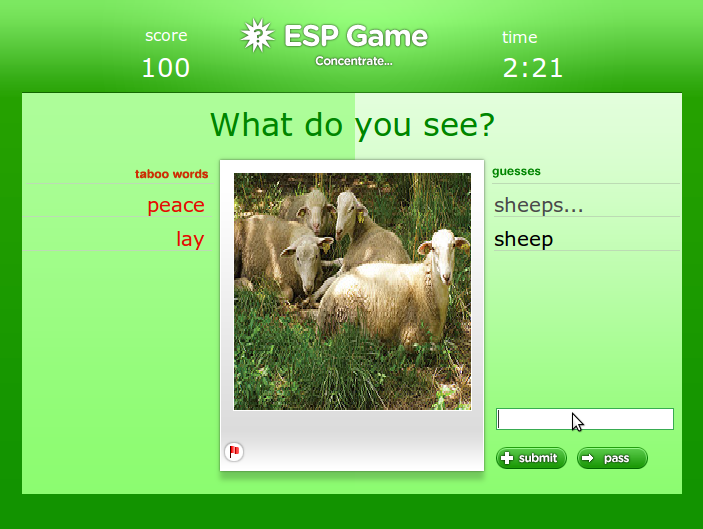
\includegraphics[width=0.5\columnwidth]{assets/img/esp.png}
\caption{Screenshot of the ESP game, by Luis Von Ahn~\cite{von2005esp}}%
\label{fig:esp}
\end{figure}

There exists another well-known mean to gather data in an implicit way: CAPTCHAs.
The term has been originally coined by
Luis Von Ahn (again) et al.~\cite{von2003captcha} and stands for
Completely Automated Public Turing Test to Tell Computer and Humans Apart.
CAPTCHAs have been created to stop automated attacks on websites,
to prevent automated creation of millions of malicious email accounts.
The idea is to create a Turing test~\cite{machinery1950computing},
i.e.\ a test that a human should be able to complete effortlessly
while a machine would be unable to perform it.
Original versions of CAPTCHAs displayed distorted,
geometrically transformed words which would make it unrecognizable
by standard optical character recognition (OCR) softwares.
The task remained fairly easy to humans,
and required in average 13s~\cite{von2008recaptcha}.
At the time, ambitious projects were ran in parallel to digitize
tremendous collections of books, like \textit{Google Books},
which makes available searching through millions of books.
This process of digitizing books was automated using OCR softwares,
but failed for 20\% of the words in older books due to faded ink for example.
The reCAPTCHA system offers a clever way to match the two very different
problems of securing websites and digitizing old books by proposing words from old books,
that could not be recognized automatically,
to humans who wish to use an online service and are perfectly able to recognize them.
The authors report that in 2008, after one year of deployment,
reCAPTCHA has helped decipher 440M words, which amounts for more than 17,000 books.

\begin{figure}
	\centering
	\begin{tabular}{ccc}
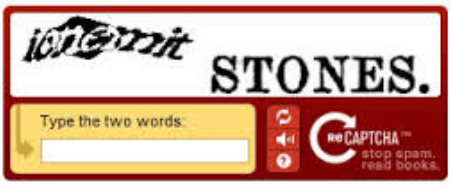
\includegraphics[width=5cm]{assets/img/recaptcha.png} & 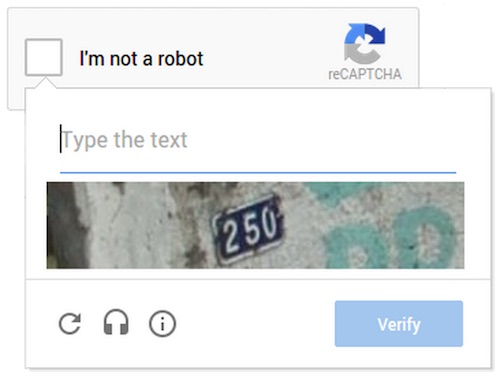
\includegraphics[width=4cm]{assets/img/recaptcha-streetview.jpg} &
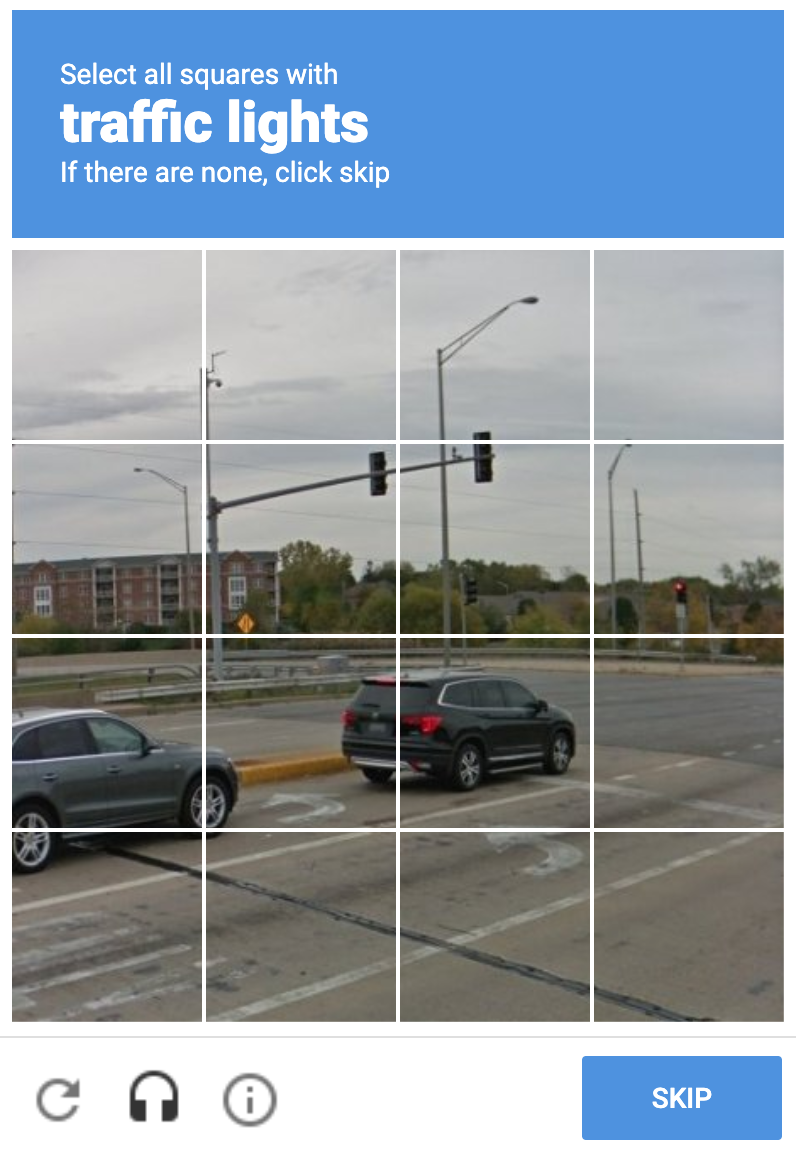
\includegraphics[width=3cm]{assets/img/reCAPTCHA_v2.png} \\
	\end{tabular}
	\caption{Screenshots illustrating the evolution of reCAPTCHA~\cite{von2008recaptcha} tasks over the years.}%
	\label{fig:recaptcha}
\end{figure}

While there are no further publications on reCAPTCHA,
one has been able to observe its evolution through the years (see figure~\ref{fig:recaptcha}).
Driven by the need to come up with problems that still resist computers,
it went from text to image recognition, from digit recognition
in pictures probably extracted from \textit{Google Street View} to object detection
in urban scenes pictures, very likely to target autonomous vehicles applications.

\subsection{Expert vs.\ non-expert annotators}

Whether they are implicit or explicit,
annotations need to be performed by human annotators and
there have been several trends throughout the years.
In essence, we could split annotators into two sets of users:
experts, from whom we can expect high quality annotations
but are rare and expensive, and non-expert users
who tend to make more mistakes but provide much cheaper annotations.

Historically, the first datasets of reasonable scale which are PASCAL and CIFAR,
did not require too many annotators.
In fact, the authors of PASCAL~\cite{Everingham10} reported that a ``party'' of users
annotated the images after an initial training.
They were probably students, but no details are provided as to how many of them.
These users were also regularly observed during annotations
to ensure the quality of their work.
Finally, one of the organizers of the PASCAL challenge checked all the annotations.
Similarly, the CIFAR dataset~\cite{krizhevsky2009learning}
was labelled by a group of students paid for the task.

With time, there was a demand for larger datasets.
They aimed at expanding the number of classes,
as well as the number of annotated images.
With this new goal in mind,
the dataset authors started \textit{crowdsourcing} the annotations.
Crowdsourcing is a process in which a task that should usually be performed
by an expert is outsourced to a crowd of non-expert users.
The term was first coined by Jeff Howe in 2006~\cite{howe2006rise}.
The creation of specific online platforms
such as Amazon Mechanical Turk or Crowdflower
considerably eased the process of crowdsourcing image annotation.
ImageNet and MS COCO have both been annotated by Turkers,
i.e.\ humans recruited and paid through Amazon Mechanical Turk.
Since the difficulty to clearly instruct remote users is increased,
the annotations interfaces need to be carefully designed,
and the annotation quality need to be properly ensured;
this will be described in Section~\ref{sec:annotation_quality}.

While crowdsourcing is widely used, it may not be relevant to all setups.
In cases when images are sensitive for example,
it is not possible to outsource the annotation process outside of a company.
In addition, the need for redundancy to ensure annotation quality
limits the positive impact on cost that crowdsourcing is supposed to provide.
Although being one of the largest annotated dataset,
Open Images has been for the most part annotated by in-house employees at Google.
To achieve this, interactions have been specially designed to lead
to good annotations in a faster way.
For example, extreme clicking for bounding box annotations~\cite{papadopoulos2017extreme}
introduces a clever interaction that allows to draw bounding boxes more quickly,
avoiding the errors that usually force users to start over.
Alternatively, the authors of~\cite{OpenImagesSegmentation}
propose an interactive segmentation algorithm in which user clicks
guide a deep neural network and refine the segmentation mask.
The images can be annotated 3 times faster than when
using a standard polygon drawing tool such as with LabelMe~\cite{russell2008labelme},
and the segmentation boundaries are much more precise.
We present a similar contribution in the next chapter.


\subsection{Quality check of annotations}%
\label{sec:annotation_quality}

As stated in the previous section, crowdsourcing is currently one of
the leading methods to gather annotations for creating image datasets.
However, and while the annotations come at a relative cheap cost,
the quality of the collected data is often questionable.
Oleson et al.~\cite{oleson2011programmatic} have classified
three categories of errors that non-expert users are likely to commit
when performing Human Intelligence Tasks
(HIT), the term coined in Amazon Mechanical turk to designate the micro-jobs offered to the users.
The first source of errors, called \textit{unsufficient attention} by Oleson,
simply occurs when the humans enrolled to perfom HITs, called workers,
make occasional mistakes, due to the task complexity or a lack of attention for example.
Some other workers, called \textit{incompetent} by Oleson,
may not understand the task and behave unpredictably.
The data they provide is often unusable.
Finally, a last class of workers, called \textit{scammers},
designates users who try to trick the system to collect the reward.
A good quality checking process should account for these three types of possible errors.
Oleson et al.\ point out the advantages of adding gold standard images
i.e.\ images for which a ground-truth annotation is known,
among the data to be able to estimate workers reliability.
The authors of ImageNet~\cite{ILSVRC15} also reported using this technique.
Using gold standard is a good practice to detect scammers and incompetent workers.

\begin{figure}[ht]
\centering
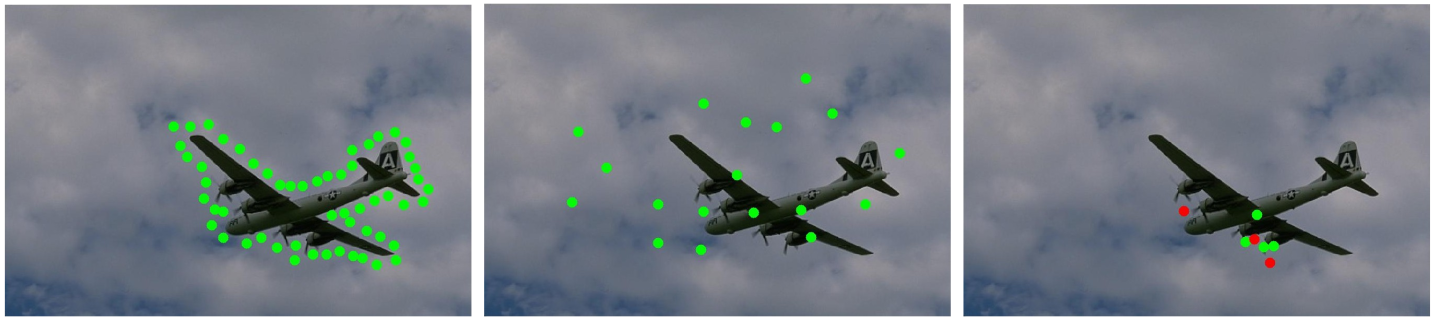
\includegraphics[width=\columnwidth]{assets/img/crowdsourcing-errors.png}
\caption{Illustration of possible mistakes that happen during
	a crowdsourcing campaign~\cite{carlier2016assessment}:
	on the left, annotations from a user who misunderstood the task,
	to be compared with the expected results on the right
	(red points on the background, green points on the foreground).
	In the middle, annotation of a \textit{scammer}.}%
\label{fig:cs-errors}
\end{figure}

The most obvious way to detect workers mistakes
is to introduce redundancy in the annotations.
Multiple workers are tasked to label the same image,
and the annotations are validated if they are similar enough.
This straightforward strategy has been formalized by Luis Von Ahn~\cite{von2008designing}
under the term \textit{output agreement}:
multiple users agree on the same output annotation for a given image.
Authors of MS COCO~\cite{lin2014microsoft}
report asking up to 8 workers to perform the same task,
for example to increase the recall in an instance spotting task.
Redundancy helps reducing the impact of unsufficient attention.


Another technique to prevent
having too many incompetent workers is
to go through a tutorial before starting the task.
Gottlieb et al.~\cite{gottlieb2012pushing} have shown
that the performance of users who complete a tutorial beforehand
is significantly higher than users who did not.
In~\cite{lin2014mscoco}, users are filtered
based on their performance in an initial training task
and are periodically verified during the whole annotation process.


The error rate can also be limited by a clever labor division.
A Human Intelligence Task should always be an atomic operation,
simple to explain and quick to perform.
For example, the authors of~\cite{su2012crowdsourcing} introduce
a Find-Fix-Verify pattern for object detection annotations.
Output agreement is difficult to implement for bounding boxes
due to the the presence of thresholds to measure similarity.
Therefore, the authors introduce a series of micro-tasks
ensuring the quality of the final bounding boxes.
A first group of workers is tasked to draw bounding boxes (\textit{Find}),
and a second group of different workers is asked to validate
each of the bounding boxes (\textit{Fix}).
Being a binary decision,
it is easier to implement output agreement on this second task.
Finally a last group of users is in charge of checking whether
some objects have been omitted by the first pool of workers (\textit{Verify}).
Another example of work division is described
in~\cite{chen2015microsoft} for instance segmentation.
Four different tasks are defined and sequentially operated by different workers:
image labelling (\textit{Which objects appear in the image?}),
instance spotting (users should click on each instance of a particular object),
instance segmentation, and segmentation verification.
Redundancy is introduced at every step except for the third one,
which is the more time-consuming and is especially verified by the fourth task.


A final control of the annotations quality can be done at the end of the study.
This is an approach adopted in PASCAL~\cite{Everingham10} for example,
but also in Open Images~\cite{OpenImages} in which the expert annotators
verify automatically derived labels, obtained through deep learning.


\subsection{Annotation interaction usability}

A common feature of all the points we have discussed
in the three previous sections is that the goal of the annotation process
is to obtain the largest possible number of annotations,
of the highest possible quality, and at the lowest possible cost.
Implicit annotation is cheaper but often difficult to put into place in practice.
Expert annotators provide reliable annotations but are expensive,
whereas a large number of less precise annotations can come
at a cheaper cost when using crowdsourcing.
Quality check helps ensuring annotations reliability but introduce new expenses.


With that goal in mind, there also exists another variable
which is rarely taken into account: the usability of the annotation interaction.
Usability is a computer-human interaction concept
that has been defined by Nielsen~\cite{nielsen1994usability}.
In essence, it describes the extent to which an interface
can be mastered and used to efficiently perform the task it has been designed for.
Nielsen also introduces five criteria that help measuring an interface usability:
subjective satisfaction, easiness to learn and to remember,
efficiency with respect to a certain task, and error robustness.
It is really interesting to note that all of these criteria
are relevant to image annotation;
we want the users to be efficient, i.e.\ to provide good annotations
in the minimum amount of time.
We want the users to make as few errors as possible,
and we also want them to easily learn and remember their task, once again, to be cost-effective.
While usability is a core concept of computer human interaction,
very few of the annotation tools that we described previously mention they want to optimize it.


Korinke et al.~\cite{korinke_intuitive_2015,korinke_exploring_2015}
have studied how touch devices should be used to perform image segmentation.
They compare several types of interactions and conduct
two user studies to evaluate and compare these interactions.
More recently, and while usability is not explicity mentioned,
the work of Papadopoulos et al.~\cite{papadopoulos2017extreme}
on extreme clicking is particularly interesting.
The goal the work is two-fold: reducing the annotator cognitive load
and improving the quality of the annotations.
The authors propose replacing the traditional bounding box drawing
by clicking four extreme points (top, down, left and right)
of the object and deriving the bounding box from these points.
This interaction offers an interesting advantage:
it reduces the time needed to appropriately draw a bounding box by a factor of 5.
Users otherwise tend to start over multiple times due to the non-convexity of objects shape.
It also provides richer annotations as four points lying on the object boundary are provided;
the authors take advantage of this property to generate reasonable quality segmentations
from this very weak information of only four points.
Some subsequent work of the same group adopt similar approaches for image segmentation,
providing users with the ability to correct segmentations
by scribbling~\cite{agustsson2018interactive} or clicking~\cite{OpenImagesSegmentation}.


\section{Different types of interactions for image annotation}%
\label{sec:annotation-types}
In this section, we briefly review and analyze the interactions that have been used for image annotation.

Directly related to image classification and image captioning
is the simple interaction of \textit{free text typing}.
It often consists of a single text box in which the annotator can type a word,
a set of words, or even complete sentences.
This annotation can be associated to the entire image, like for image captioning

\begin{itemize}
	\item Free text typing
	\item Icon clicking
	\item points, lines
	\item bounding box
	\item polygon
	\item circles, ellipses?
\end{itemize}

THE BIG TABLe: datasets and relevant papers, to be classified
